\documentclass{article}
\usepackage{geometry}
\usepackage{graphicx}
\usepackage{subcaption}
\usepackage{amsmath}
\usepackage{booktabs}

\title{Structure from Motion Project Report}
\author{Pooya Nasiri \thanks{Email: pooya.nasiri@studenti.unipd.it | Matricola 2071437} \and Rajmonda Bardhi \thanks{Email: rajmonda.bardhi@studenti.unipd.it | Matricola 2071810}}
\date{May 15, 2024}

\begin{document}

\maketitle

\section*{Contributions}
\noindent \textbf{Pooya Nasiri:}
\begin{itemize}
    \item Feature Extraction and Matching: We extracted salient points and descriptors from images and performed exhaustive matching between image pairs.
    \item Triangulation of 3D Points: Triangulating 3D points from pairs of observations allowed us to reconstruct the scene geometry.
    \item Residual Block Addition: We incorporated residual blocks into the Ceres Solver problem to iteratively improve reconstruction accuracy.
\end{itemize}

\noindent \textbf{Rajmonda Bardhi:}
\begin{itemize}
    \item Initial Rigid Body Transformation: We estimated the initial rigid body transformation between image pairs to identify suitable seed pairs for reconstruction.
    \item Auto-Differentiable Cost Function: Implementing an auto-differentiable cost function was crucial for optimizing camera parameters and 3D point positions.
    \item Reconstruction Divergence Detection: Mechanisms were developed to detect reconstruction divergence, safeguarding against incorrect reconstructions.
\end{itemize}

\section{Introduction}

Structure from Motion (SfM) is a fundamental technique in computer vision, enabling the reconstruction of 3D scenes from 2D images. In this project, we develop a robust SfM pipeline aimed at reconstructing real-world scenes accurately. Through the integration of various algorithms, we address challenges such as feature extraction, camera pose estimation, and 3D point triangulation. By delving into the intricacies of SfM, we aim to gain insights into 3D data processing and computer vision applications. This project serves as a platform to explore the principles of SfM and its practical implications for scene reconstruction.


\section{Features Matcher}
\subsection{Extracting Salient Points, Descriptors, and Feature Colors}
The \texttt{extractFeatures()} function in the \texttt{FeatureMatcher} class processes a set of images to extract salient points, descriptors, and feature colors. Here's a breakdown of the implementation:

\begin{itemize}
  \item It initializes vectors to store features (\texttt{features\_}), descriptors (\texttt{descriptors\_}), and feature colors (\texttt{feats\_colors\_}) for each image.
  \item Utilizes the ORB (Oriented FAST and Rotated BRIEF) feature detector and descriptor extractor provided by OpenCV.
  \item For each image:
    \begin{itemize}
      \item Reads the image.
      \item Detects keypoints using the ORB feature detector.
      \item Computes descriptors for the detected keypoints.
      \item Stores the keypoints and descriptors in the respective vectors.
      \item Extracts the color information of each feature by accessing the corresponding pixel in the image and stores it in the \texttt{feats\_colors\_} vector.
    \end{itemize}
\end{itemize}

This function serves as the initial step in the Structure from Motion pipeline, providing essential input data for subsequent tasks such as feature matching and geometric verification.


\subsection{Matching Descriptors Between Images}

The \texttt{exhaustiveMatching()} function in the \texttt{FeatureMatcher} class matches descriptors between images and performs geometric validation. Here's a breakdown of the implementation:

\begin{itemize}
  \item It initializes vectors to store raw matches and inlier matches.
  \item For each pair of images:
    \begin{itemize}
      \item Matches descriptors between image $i$ and image $j$ using a brute-force matcher 
      
      (\texttt{cv::BFMatcher}).
      \item Estimates the Essential matrix and filters matches to obtain inlier matches using 
      
      \texttt{cv::findEssentialMat()} with RANSAC.
      \item Checks if the number of inlier matches is sufficient.
      \item If enough inliers are found, estimates the Homography matrix and filters matches again to obtain inlier matches.
      \item Checks if the number of inlier matches for the Homography matrix is sufficient.
      \item Sets the inlier matches if the number of inliers is satisfactory using the \texttt{setMatches()} function.
    \end{itemize}
\end{itemize}

This function plays a crucial role in the Structure from Motion pipeline by establishing correspondences between keypoints in different images and filtering out unreliable matches based on geometric validation.
This section provides a clear overview of how descriptors are matched between images and validated geometrically to ensure the accuracy of correspondences.


\section{Basic SFM}
\subsection{Extracting Essential Matrix and Homography Matrix}
The code snippet provides an implementation to extract both the Essential matrix ($E$) and the Homography matrix ($H$), followed by the validation of these matrices to determine the suitability of the seed pair for further processing. Here's a breakdown of the implementation:

\begin{itemize}
  \item Estimates the Essential matrix ($E$) and the Homography matrix ($H$) using RANSAC.
  \item Checks if the number of inliers for the Essential matrix ($E$) is higher than the number of inliers for the Homography matrix ($H$). If not, it returns false, indicating that the seed pair is not suitable, and a new pair needs to be tried.
  \item If the number of inliers for $E$ is higher than for $H$, it recovers the initial rigid body transformation between the seed pair indices ($seed\_pair\_idx0$ and $seed\_pair\_idx1$) from the Essential matrix using the \texttt{cv::recoverPose()} function.
  \item Checks if the recovered transformation is mainly given by a sideward motion, which is preferred over forward motion. If not, it returns false.
  \item If the motion is primarily sideward, it stores the transformation in $init\_r\_mat$ and $init\_t\_vec$.
\end{itemize}

This section is crucial for determining the quality of the seed pair and extracting the initial rigid body transformation, which is essential for further steps in the Structure from Motion process. And provides a detailed explanation of how the Essential and Homography matrices are extracted and validated within the Structure from Motion pipeline.


\subsection{Triangulating New 3D Points from 2D Projections}

The code segment aims to triangulate new 3D points based on observations from different camera poses. It performs the following steps:

- Iterates over camera poses and their corresponding observations.
- For each observation:
  - Checks if the camera pose has been optimized.
  - Ensures that the point has not been optimized yet and is observed in both the new camera pose and another camera pose.
  - Triangulates the 3D point using observations from both camera poses.
  - Validates the chirality constraint to ensure the triangulated point is located in front of both cameras.
  - Updates the point data if the chirality constraint is satisfied.

This section is vital for augmenting the reconstruction with new 3D points, leveraging observations from multiple camera poses.



\subsection{Implementing Auto-Differentiable Cost Function}

The code defines a struct named \texttt{ReprojectionError}, which serves as an auto-differentiable cost function. Here's a breakdown of the implementation:

- The struct includes an \texttt{operator()} method, which computes the residuals between observed and projected points.
- Inside the \texttt{operator()} method:
  - It extracts camera parameters (rotation and translation) and projects the 3D point into the image plane using the normalized, canonical camera model.
  - Residuals are computed as the difference between normalized projected points and observed points.
- It provides a static \texttt{Create} method to create a \texttt{ceres::CostFunction} using automatic differentiation provided by Ceres Solver.
- The cost function is templated with two sets of parameters: 6 parameters for camera (rotation and translation) and 3 parameters for the 3D point.

This struct is crucial for defining the cost function used in the optimization process, allowing for automatic differentiation and efficient optimization of camera parameters and 3D points.


\subsection{Adding Residual Blocks to Ceres Solver Problem}

The code segment adds residual blocks to the Ceres Solver problem for each observation that has been registered. Here's a breakdown of the implementation:

- It initializes a Ceres Solver problem and saves a copy of the initial parameters.
- For each observation:
  - It checks if the observation has already been registered, both in terms of camera pose and point position.
  - If the observation is registered:
    - It adds a residual block to the problem.
    - The residual block is defined using the \texttt{ReprojectionError} functor, as seen in the provided code snippet.
    - The residual block incorporates a Cauchy loss function with parameters, typically chosen as 2 times the maximum reprojection error (\texttt{max\_reproj\_err}).
    - The parameters for the camera pose and point position are retrieved using the \texttt{cameraBlockPtr()} and \texttt{pointBlockPtr()} functions, respectively.
    - The residual block is added to the problem using the \texttt{AddResidualBlock()} method.

This section is essential for formulating the optimization problem in Ceres Solver, incorporating residuals based on observed and projected points.


\subsection{Detecting Reconstruction Divergence}

The code snippet is responsible for detecting if the reconstruction process has diverged. Here's how it works:

- It checks for potential divergence by comparing the previous and updated camera parameters, as well as the point positions.
- For each camera pose:
  - It compares the previous camera parameters (\texttt{prev\_camera}) with the updated camera parameters (\texttt{updated\_camera}).
  - If any parameter differs by more than a predefined threshold (\texttt{divergence\_threshold}), it flags the reconstruction as diverged.
- Similarly, it checks for divergence in point positions:
  - It compares the previous point parameters (\texttt{prev\_pts}) with the updated point parameters (\texttt{updated\_pts}).
  - If any point parameter differs significantly from its previous value, it flags the reconstruction as diverged.
- If divergence is detected in either camera parameters or point positions, the function returns false, indicating the need to reset the reconstruction and start over with a new pair of seeds.

This section is crucial for ensuring the integrity of the reconstruction process by detecting and handling potential divergence scenarios.

\newpage
\section{Results}

The results showcase the effectiveness of the implemented SfM pipeline in reconstructing 3D scenes from 2D images. Sample screenshots of output results for different datasets are presented.

\begin{figure}[h]
    \centering
    \begin{subfigure}[b]{0.32\textwidth}
        \centering
        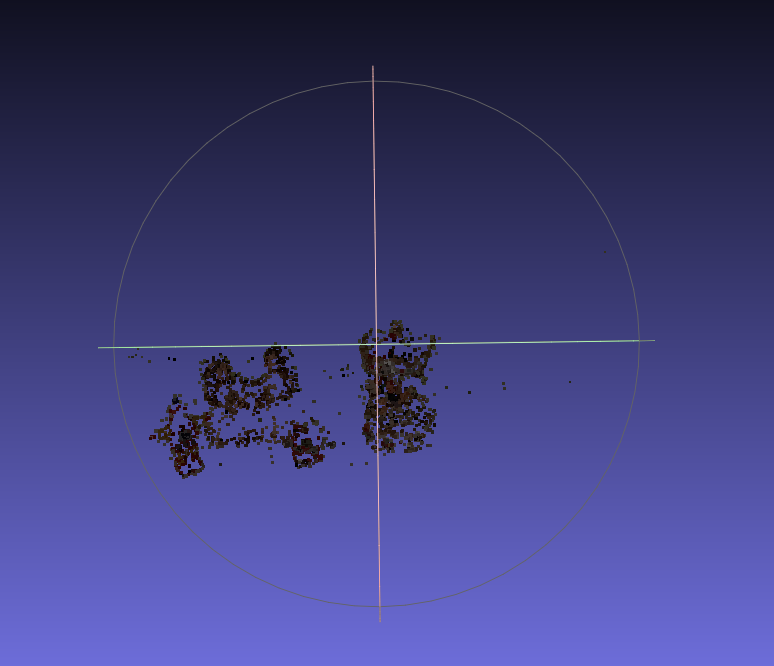
\includegraphics[width=\textwidth]{1.png}
        \caption{Sample screenshot of output result for first dataset (Dolls)}
    \end{subfigure}
    \hfill
    \begin{subfigure}[b]{0.32\textwidth}
        \centering
        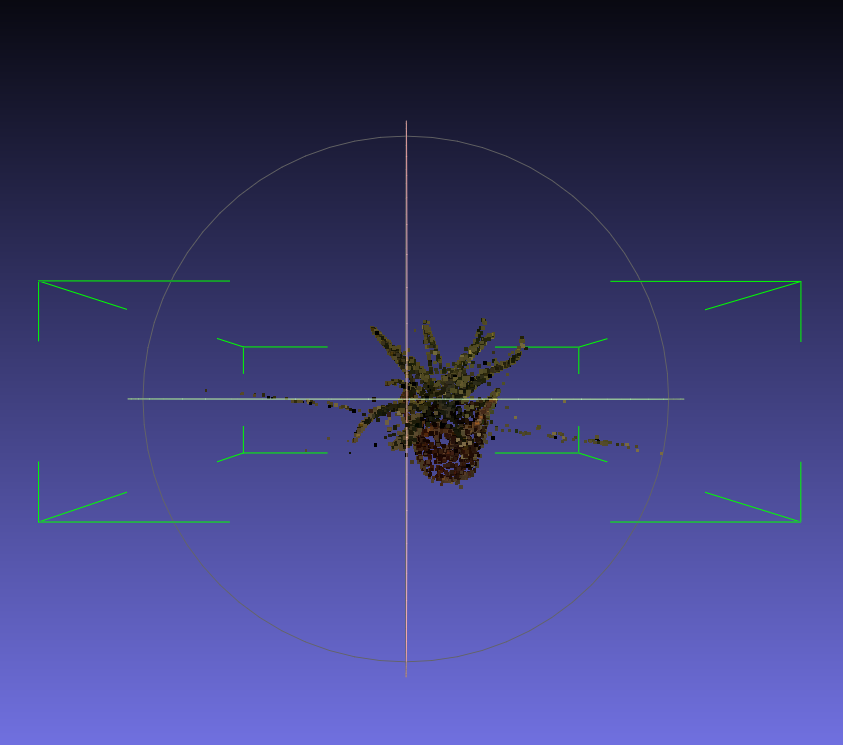
\includegraphics[width=\textwidth]{2.png}
        \caption{Sample screenshot of output result for second dataset (Vase)}
    \end{subfigure}
    \hfill
    \begin{subfigure}[b]{0.32\textwidth}
        \centering
        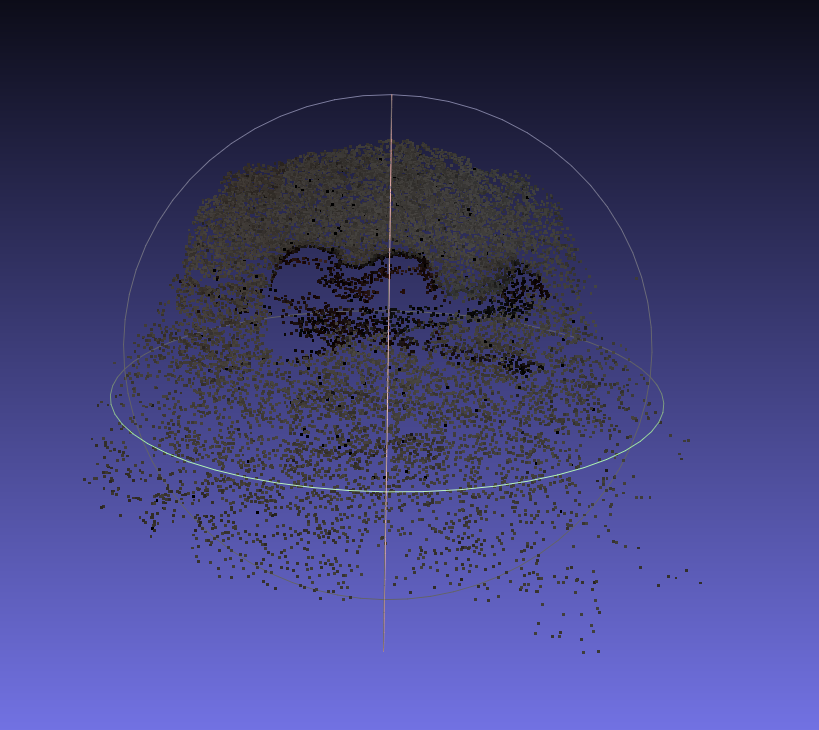
\includegraphics[width=\textwidth]{3.png}
        \caption{Sample screenshot of output result for third dataset (Violin)}
    \end{subfigure}
    \caption{Sample screenshots of output results for different datasets}
\end{figure}

During the project, a common error encountered was: "DLT algorithm needs at least 6 points for pose estimation from 3D-2D point correspondences. (expected: 'count $\geq$  6')."


\section{Conclusion}

Throughout this project, our goal was to develop a robust Structure from Motion (SfM) pipeline for reconstructing 3D scenes from 2D images. Divided into seven key tasks, our approach addressed critical aspects of the SfM pipeline:

\begin{enumerate}
\item \textbf{Feature Extraction and Matching:} We extracted salient points and descriptors from images and performed exhaustive matching between image pairs. This step was fundamental in identifying correspondences across images, forming the basis for subsequent tasks. By utilizing the ORB feature detector and descriptor extractor, we ensured efficient and reliable feature detection and matching.

\item \textbf{Initial Rigid Body Transformation:} We estimated the initial rigid body transformation between image pairs to identify suitable seed pairs for reconstruction. This transformation was essential for establishing a coherent starting point for the 3D reconstruction process. Accurate initial estimates helped in reducing errors in the final 3D model.

\item \textbf{Triangulation of 3D Points:} Triangulating 3D points from pairs of observations allowed us to reconstruct the scene geometry. This process involved calculating the 3D positions of points by finding the intersection of lines of sight from multiple images. The precision of triangulation directly impacted the accuracy of the reconstructed 3D model.

\item \textbf{Auto-Differentiable Cost Function:} Implementing an auto-differentiable cost function was crucial for optimizing camera parameters and 3D point positions. This function enabled gradient-based optimization methods, allowing for more precise adjustments of the model parameters. The use of automatic differentiation simplified the implementation of complex optimization algorithms.

\item \textbf{Residual Block Addition:} We incorporated residual blocks into the Ceres Solver problem to iteratively improve reconstruction accuracy. These residual blocks represented the differences between observed and predicted values, guiding the optimization process to minimize reconstruction errors. Iterative refinement through residuals enhanced the overall quality of the 3D model.

\item \textbf{Reconstruction Divergence Detection:} Mechanisms were developed to detect reconstruction divergence, safeguarding against incorrect reconstructions. These mechanisms monitored the consistency and reliability of the reconstruction process, identifying potential issues early and preventing the propagation of errors. Ensuring stability in the reconstruction pipeline was critical for producing accurate and reliable 3D models.
\end{enumerate}

Our comprehensive SfM pipeline offers versatility in reconstructing scenes with varying complexities. By addressing key components such as feature extraction, initial transformation, triangulation, optimization, and error detection, we created a robust framework capable of handling diverse datasets. 

Further optimizations and enhancements, such as bundle adjustment and loop closure, could improve reconstruction accuracy and robustness. Bundle adjustment would refine the 3D structure and camera parameters by minimizing re-projection errors across all images, while loop closure would enhance the ability to handle large-scale scenes by detecting and correcting loop-related errors.

In summary, this project lays the groundwork for future advancements in 3D data processing and computer vision applications. The developed SfM pipeline not only demonstrates the feasibility of accurate 3D reconstruction from 2D images but also provides a scalable foundation for further research and development in the field of computer vision.

\end{document}
